% fig_transfer_topology.tex
% Five busbar transfer topologies (T1--T5) shown as state-machine
% horizontal strip with zone assignment annotations
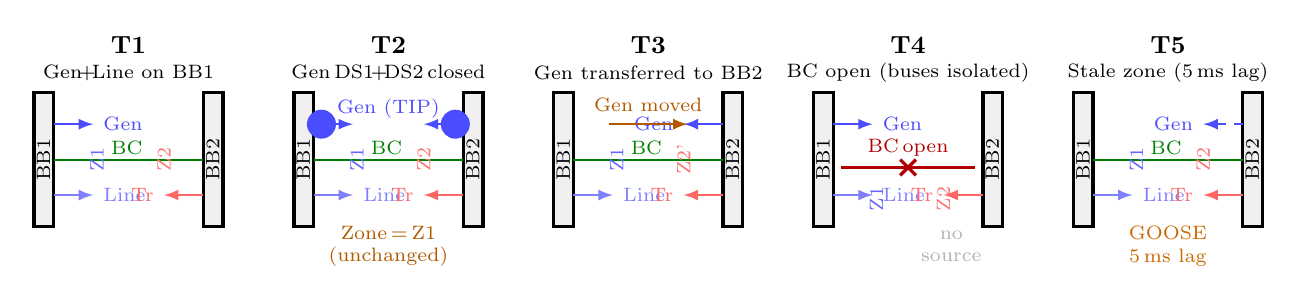
\begin{tikzpicture}[
  bb/.style={draw, fill=gray!12, minimum width=22pt, minimum height=70pt,
             line width=1.2pt},
  feeder/.style={draw, thick, -latex},
  flab/.style={font=\scriptsize},
  tlab/.style={font=\small\bfseries},
  ds/.style={draw, circle, fill=white, inner sep=1.5pt, font=\tiny},
  arrow/.style={-latex, thick, orange!70!black},
  ]

% ============================================================
% Row layout: 5 topologies side by side
% Spacing: each topology block is 3.0 cm wide
% ============================================================

\foreach \topo/\tlabel/\desc/\xoff in {
  T1/T1\,NORM/Gen\!+\!Line on BB1/0,
  T2/T2\,TIP/Gen\,DS1\!+\!DS2\,closed/3.3,
  T3/T3\,POST/Gen transferred to BB2/6.6,
  T4/T4\,SPLIT/BC open (buses isolated)/9.9,
  T5/T5\,LAG/Stale zone (5\,ms lag)/13.2
} {
  % Topology label
  \node[tlab] at (\xoff+1.4, 3.3) {\topo};
  \node[flab, align=center] at (\xoff+1.4, 2.95) {\desc};

  % BB1 busbar
  \draw[bb] (\xoff+0.2, 1.0) rectangle (\xoff+0.45, 2.7);
  \node[flab, rotate=90] at (\xoff+0.32, 1.85) {BB1};

  % BB2 busbar
  \draw[bb] (\xoff+2.35, 1.0) rectangle (\xoff+2.6, 2.7);
  \node[flab, rotate=90] at (\xoff+2.47, 1.85) {BB2};
}

% ============================================================
% T1_NORM: Gen(BB1), Line(BB1), Tr(BB2), BC(closed)
% ============================================================
\def\x{0}
% Gen $\to$ BB1
\draw[feeder, blue!70] (\x+0.45, 2.3) -- ++(0.5,0) node[right, flab, blue!70]{Gen};
% Line $\to$ BB1
\draw[feeder, blue!50] (\x+0.45, 1.4) -- ++(0.5,0) node[right, flab, blue!50]{Line};
% BC (closed)
\draw[thick, green!50!black] (\x+0.45, 1.85) -- (\x+2.35, 1.85);
\node[flab, green!50!black] at (\x+1.40, 2.00) {BC\,\checkmark};
% Tr $\to$ BB2
\draw[feeder, red!60] (\x+2.35, 1.4) -- ++(-0.5,0) node[left, flab, red!60]{Tr};
% Zone labels
\node[flab, blue!60, rotate=90] at (\x+1.0, 1.85) {Z1};
\node[flab, red!55,  rotate=90] at (\x+1.85, 1.85) {Z2};

% ============================================================
% T2_TIP: Gen has BOTH DS closed (both lines to BB1 and BB2)
% ============================================================
\def\x{3.3}
% Gen $\to$ BB1 (solid) + BB2 (dashed)
\draw[feeder, blue!70] (\x+0.45, 2.3) -- ++(0.5,0);
\draw[blue!70, dashed, thick, -latex] (\x+2.35, 2.3) -- ++(-0.5,0);
\node[flab, blue!70] at (\x+1.4, 2.5) {Gen (TIP)};
% DS circles on Gen
\node[ds, blue!70] at (\x+0.55, 2.3) {C};
\node[ds, blue!70] at (\x+2.25, 2.3) {C};
% Line $\to$ BB1
\draw[feeder, blue!50] (\x+0.45, 1.4) -- ++(0.5,0) node[right, flab, blue!50]{Line};
% BC (closed)
\draw[thick, green!50!black] (\x+0.45, 1.85) -- (\x+2.35, 1.85);
\node[flab, green!50!black] at (\x+1.40, 2.00) {BC\,\checkmark};
% Tr $\to$ BB2
\draw[feeder, red!60] (\x+2.35, 1.4) -- ++(-0.5,0) node[left, flab, red!60]{Tr};
% Zone labels (unchanged during TIP)
\node[flab, blue!60, rotate=90] at (\x+1.0, 1.85) {Z1};
\node[flab, red!55,  rotate=90] at (\x+1.85, 1.85) {Z2};
% TIP annotation
\node[flab, orange!70!black, align=center] at (\x+1.4, 0.75)
  {Zone\,=\,Z1\\(unchanged)};

% ============================================================
% T3_POST: Gen transferred to BB2
% ============================================================
\def\x{6.6}
% Gen $\to$ BB2 (now on BB2)
\draw[feeder, blue!70] (\x+2.35, 2.3) -- ++(-0.5,0) node[left, flab, blue!70]{Gen};
% Line $\to$ BB1
\draw[feeder, blue!50] (\x+0.45, 1.4) -- ++(0.5,0) node[right, flab, blue!50]{Line};
% BC (closed)
\draw[thick, green!50!black] (\x+0.45, 1.85) -- (\x+2.35, 1.85);
\node[flab, green!50!black] at (\x+1.40, 2.00) {BC\,\checkmark};
% Tr $\to$ BB2
\draw[feeder, red!60] (\x+2.35, 1.4) -- ++(-0.5,0) node[left, flab, red!60]{Tr};
% Zone labels (reconfigured)
\node[flab, blue!60, rotate=90] at (\x+1.0, 1.85) {Z1};
\node[flab, red!55,  rotate=90] at (\x+1.85, 1.85) {Z2'};
% Arrow showing Gen moved
\draw[arrow] (\x+0.90, 2.30) -- (\x+1.90, 2.30);
\node[flab, orange!70!black] at (\x+1.4, 2.55) {Gen moved};

% ============================================================
% T4_SPLIT: BC open
% ============================================================
\def\x{9.9}
% Gen $\to$ BB1
\draw[feeder, blue!70] (\x+0.45, 2.3) -- ++(0.5,0) node[right, flab, blue!70]{Gen};
% Line $\to$ BB1
\draw[feeder, blue!50] (\x+0.45, 1.4) -- ++(0.5,0) node[right, flab, blue!50]{Line};
% BC OPEN (red X)
\draw[red!70!black, thick] (\x+0.55, 1.75) -- (\x+2.25, 1.75);
\draw[red!70!black, very thick] (\x+1.3, 1.65) -- (\x+1.5, 1.85);
\draw[red!70!black, very thick] (\x+1.3, 1.85) -- (\x+1.5, 1.65);
\node[flab, red!70!black] at (\x+1.40, 2.00) {BC\,open};
% Tr $\to$ BB2
\draw[feeder, red!60] (\x+2.35, 1.4) -- ++(-0.5,0) node[left, flab, red!60]{Tr};
% Zone labels
\node[flab, blue!60, rotate=90] at (\x+1.0, 1.35) {Z1};
\node[flab, red!55,  rotate=90] at (\x+1.85, 1.35) {Z2};
% No-source annotation on BB2
\node[flab, gray!60, align=center] at (\x+1.95, 0.75) {no\\source};

% ============================================================
% T5_LAG: POST topology, stale NORM zone
% ============================================================
\def\x{13.2}
% Gen $\to$ BB2 (actual)
\draw[feeder, blue!70, dashed] (\x+2.35, 2.3) -- ++(-0.5,0)
  node[left, flab, blue!70]{Gen};
% Line $\to$ BB1
\draw[feeder, blue!50] (\x+0.45, 1.4) -- ++(0.5,0) node[right, flab, blue!50]{Line};
% BC (closed)
\draw[thick, green!50!black] (\x+0.45, 1.85) -- (\x+2.35, 1.85);
\node[flab, green!50!black] at (\x+1.40, 2.00) {BC\,\checkmark};
% Tr $\to$ BB2
\draw[feeder, red!60] (\x+2.35, 1.4) -- ++(-0.5,0) node[left, flab, red!60]{Tr};
% Stale zone label
\node[flab, blue!60, rotate=90] at (\x+1.0, 1.85) {Z1};
\node[flab, red!55,  rotate=90] at (\x+1.85, 1.85) {Z2};
% Stale annotation
\node[flab, orange!80!black, align=center] at (\x+1.4, 0.75)
  {GOOSE\\5\,ms lag};

\end{tikzpicture}
